\documentclass[10pt,t,handout]{beamer} % handout
\usetheme{Heverlee}
\usepackage{amsmath, amssymb}
\usepackage{tikz,tikz-cd}
\usepackage{mathtools,mathbbol}
% environments
%\newtheorem{theorem}{Theorem}
%\newtheorem{proposition}[theorem]{Proposition}
%\newtheorem{lemma}[theorem]{Lemma}
%\newtheorem{corollary}[theorem]{Corollary}
%
%\theoremstyle{definition}
%\newtheorem{definition}[theorem]{Definition}
%\newtheorem*{definition*}{Definition}
%\newtheorem{remark}[theorem]{Remark}
%\newtheorem*{remark*}{Remark}
%\newtheorem{example}[theorem]{Example}
%\newtheorem*{example*}{Example}
%\newtheorem{convention}[theorem]{Convention}
%\newtheorem*{convention*}{Convention}
%\newtheorem{notation}[theorem]{Notation}
%\newtheorem*{notation*}{Notation}
%\newtheorem{question}[theorem]{Question}
%\newtheorem*{question*}{Question}

% hyphenation
\hyphenation{co-chain}
\hyphenation{co-chains}
\hyphenation{co-al-ge-bra}
\hyphenation{co-al-ge-bras}
\hyphenation{co-bound-ary}
\hyphenation{co-bound-aries}

% basics
\DeclareMathOperator{\face}{d}
\DeclareMathOperator{\dege}{s}
\DeclareMathOperator{\bd}{\partial}
\DeclareMathOperator{\sign}{sign}
\newcommand{\ot}{\otimes}
\DeclareMathOperator{\EZ}{EZ}
\DeclareMathOperator{\AW}{AW}
\newcommand{\diag}{\mathrm{D}}


% sets and spaces
\newcommand{\N}{\mathbb{N}}
\newcommand{\Z}{\mathbb{Z}}
\newcommand{\Q}{\mathbb{Q}}
\newcommand{\R}{\mathbb{R}}
\renewcommand{\k}{\Bbbk}
\newcommand{\Sym}{\mathbb{S}}
\newcommand{\Cyc}{\mathbb{C}}
\newcommand{\Ftwo}{{\mathbb{F}_2}}
\newcommand{\Fp}{{\mathbb{F}_p}}
\newcommand{\Cp}{{\mathbb{C}_p}}
\newcommand{\gsimplex}{\mathbb{\Delta}}
\newcommand{\gcube}{\mathbb{I}}

% categories
\newcommand{\Cat}{\mathsf{Cat}}
\newcommand{\Fun}{\mathsf{Fun}}
\newcommand{\Set}{\mathsf{Set}}
\newcommand{\Top}{\mathsf{Top}}
\newcommand{\CW}{\mathsf{CW}}
\newcommand{\Ch}{\mathsf{Ch}}
\newcommand{\simplex}{\triangle}
\newcommand{\sSet}{\mathsf{sSet}}
\newcommand{\cube}{\square}
\newcommand{\cSet}{\mathsf{cSet}}
\newcommand{\Alg}{\mathsf{Alg}}
\newcommand{\coAlg}{\mathsf{coAlg}}
\newcommand{\biAlg}{\mathsf{biAlg}}
\newcommand{\sGrp}{\mathsf{sGrp}}
\newcommand{\Mon}{\mathsf{Mon}}
\newcommand{\SymMod}{\mathsf{Mod}_{\Sym}}
\newcommand{\SymBimod}{\mathsf{biMod}_{\Sym}}
\newcommand{\operads}{\mathsf{Oper}}
\newcommand{\props}{\mathsf{Prop}}

% operators
\DeclareMathOperator{\free}{F}
\DeclareMathOperator{\forget}{U}
\DeclareMathOperator{\yoneda}{\mathcal{Y}}
\DeclareMathOperator{\Sing}{Sing}
\newcommand{\loops}{\Omega}
\DeclareMathOperator{\cobar}{\mathbf{\Omega}}
\DeclareMathOperator{\proj}{\pi}
\DeclareMathOperator{\incl}{\iota}

% chains
\DeclareMathOperator{\chains}{N}
\DeclareMathOperator{\cochains}{N^{\vee}}
\DeclareMathOperator{\gchains}{C}

% pair delimiters (mathtools)
\DeclarePairedDelimiter\bars{\lvert}{\rvert}
\DeclarePairedDelimiter\norm{\lVert}{\rVert}
\DeclarePairedDelimiter\angles{\langle}{\rangle}
\DeclarePairedDelimiter\set{\{}{\}}

% other
\newcommand{\id}{\mathsf{id}}
\renewcommand{\th}{\mathrm{th}}
\newcommand{\op}{\mathrm{op}}
\DeclareMathOperator*{\colim}{colim}
\DeclareMathOperator{\coker}{coker}
\DeclareMathOperator{\Med}{\mathcal{M}}
\newcommand{\Hom}{\mathrm{Hom}}
\newcommand{\End}{\mathrm{End}}
\newcommand{\coEnd}{\mathrm{coEnd}}
\newcommand{\biEnd}{\mathrm{biEnd}}
\newcommand{\xla}[1]{\xleftarrow{#1}}
\newcommand{\xra}[1]{\xrightarrow{#1}}
\newcommand{\defeq}{\stackrel{\mathrm{def}}{=}}

% letters
\newcommand{\bk}{\mathbb{k}}
\newcommand{\bF}{\mathbb{F}}

\newcommand{\sA}{\mathsf{A}}
\newcommand{\sB}{\mathsf{B}}
\newcommand{\sC}{\mathsf{C}}

\newcommand{\cA}{\mathcal{A}}
\newcommand{\cB}{\mathcal{B}}
\newcommand{\cC}{\mathcal{C}}
\newcommand{\cD}{\mathcal{D}}
\newcommand{\cE}{\mathcal{E}}

\newcommand{\cL}{\mathcal{L}}
\newcommand{\cM}{\mathcal{M}}
\newcommand{\cN}{\mathcal{N}}
\newcommand{\cO}{\mathcal{O}}
\newcommand{\cP}{\mathcal{P}}

\newcommand{\cW}{\mathcal{W}}
\newcommand{\cX}{\mathcal{X}}
\newcommand{\cY}{\mathcal{Y}}
\newcommand{\cZ}{\mathcal{Z}}

\newcommand{\rB}{\mathrm{B}}
\newcommand{\rD}{\mathrm{D}}
\newcommand{\rH}{\mathrm{H}}
\newcommand{\rP}{\mathrm{P}}
\newcommand{\rW}{\mathrm{W}}

\newcommand{\bbF}{\mathbb{F}}

% comments
\newcommand{\anibal}[1]{\textcolor{blue}{\underline{Anibal}: #1}}



\renewcommand{\Vec}{\mathsf{Vec}}
\newcommand{\HS}{\mathrm{HS}}
\newcommand{\HLC}{\mathrm{LHC}}
\newcommand{\HE}{\mathbb{H}^d}
\usepackage{csquotes}
\usepackage{pgfplots}
\usepgfplotslibrary{colormaps}
\pgfplotsset{
	compat=newest,
	colormap={mycolormap}{color=(lightgray) color=(white) color=(lightgray)}
}

\newcommand{\colorit}[1]{\textcolor{pblue}{#1}}

%%% QUICK OPTIONS:
% (A) Math font without serifs, enable line below to make math serif:
    \usefonttheme[onlymath]{serif}

% (B) Re-define primary colour by adjusting the RGB values
    %\definecolor{pblue}{RGB}{206,125,66}

% (C) Title page graphic (optional) --- this is not for the background image, see \usebackgroundtemplate to change that ---
    %\titlegraphic{\includegraphics[height=2.7cm]{example_figure.pdf}}

% (D) Add logo to bottom right-corner (optional)
    \logo{\includegraphics[height=0.7cm]{aux/icosahedron-src.pdf}\hspace{12pt}\vspace{-6pt}}

% (E) Choose one (or none) of these lines to add footline bar on all frames
    %\setbeamertemplate{footline}[infoline]  % author, title, insitute
    %\setbeamertemplate{footline}[navigation] % dots swhowing progress
    %\setbeamertemplate{footline}[navsym] % navigation symbols

% (F) Widescreen 16:9 ratio
    %\usepackage[orientation=landscape,size=custom,width=16,height=9,scale=0.45,debug]{beamerposter}

%%% TITLE PAGE INFO:

\title{Persistence in functional topology}
\subtitle{Based on work with Ulrich Bauer and Maximilian Schmahl}
\author[ammedmar]{Anibal M. Medina-Mardones}
\institute{Max Planck Institute for Mathematics in Bonn}
\date{\today}

\begin{document}
	%!TEX root = ../bgsu21.tex

{
	\usebackgroundtemplate{ \parbox[b][\paperheight][b]{\paperwidth}{\centering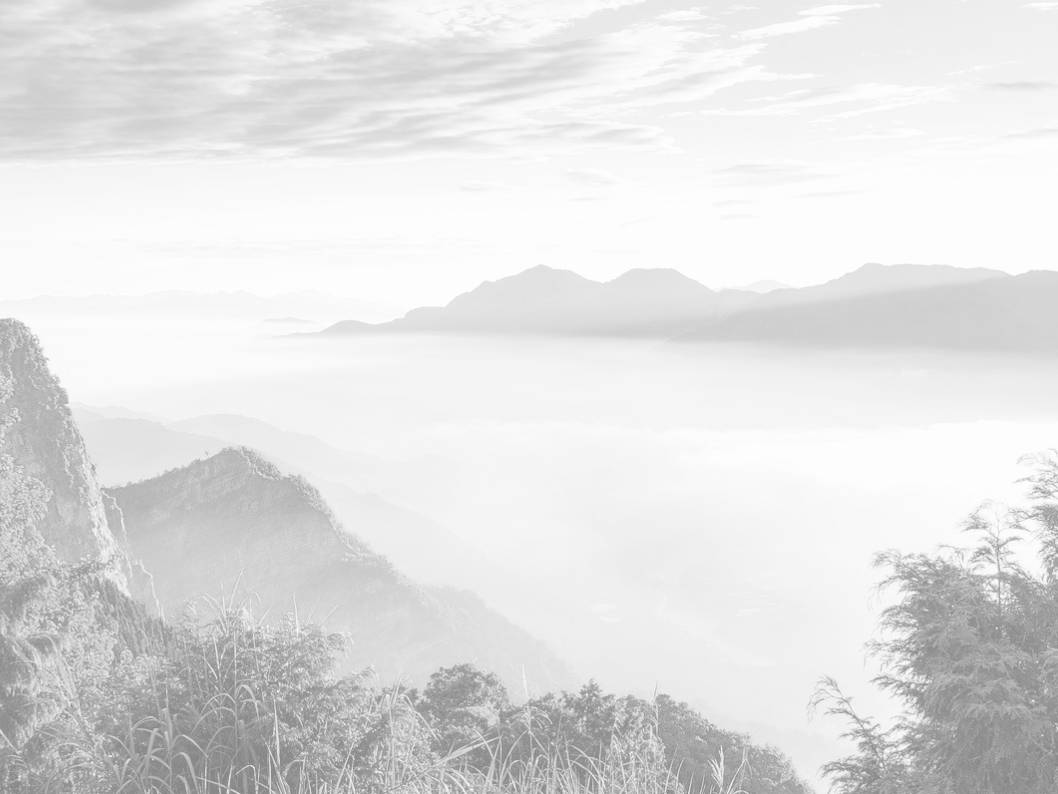
\includegraphics[width=\paperwidth]{aux/background.jpg}}}

	\setbeamercolor{background canvas}{bg=lgray}  % make background light gray

	\begin{frame}[plain,noframenumbering]
	    \titlepage
	\end{frame}
}
	%!TEX root = ../func_top.tex

\begin{frame}[plain,noframenumbering]
	\vspace*{2.3cm}
	\begin{center}
		\includegraphics[scale=.2]{aux/ukraine.pdf}
	\end{center}
\end{frame}

\begin{frame}[fragile]{Morse theory}
	\begin{center}
		\includegraphics[scale=.5]{aux/torus.pdf} \\
		\medskip
		$\downarrow f$ \\
		\medskip
		$\R \phantom{\ f}$
	\end{center}

	\pause\smallskip

	\begin{block}{Functor}
		\vspace*{-15pt}
		\[
		\begin{tikzcd}[row sep=0, column sep=small]
			(\R, \le) \arrow[r] & \Top \arrow[r] & \Vec \\
			t \arrow[r, mapsto] & f_{\leq t} \defeq f^{-1}(-\infty, t] \arrow[r, mapsto] & \rH(f_{\leq t}; \k)
		\end{tikzcd}
		\]
	\end{block}
\end{frame}

\begin{frame}[fragile]{Persistence module}
	\pause
	A \colorit{persistence module} is a functor $M \colon \R \to \Vec$.\\
	\smallskip\pause
	If $\forall t$, $\dim M_t < \infty$ It is said to be \colorit{PFD}.\\
	\smallskip\pause
	They form an Abelian category.\\
	\medskip\pause

	\colorit{Example:}
	For $I \subseteq \R$ an interval, its \colorit{interval module} is:
	\[
	C(I)_t =
	\begin{cases}
		\k, & t \in I, \\
		0, & \text{else}.
	\end{cases}
	\qquad
	C(I)_{st} =
	\begin{cases}
		\id_\R, & s,t \in I, \\
		0, & \text{else}.
	\end{cases}
	\]
	\pause\vskip-5pt
	\begin{theorem}[..., Carlssen--Zomorodian 2005, Crawley-Boevey 2015]
		For any $PFD$ persistence module $M$ there is $\set{I_\lambda \mid \lambda \in \Lambda}$ such that
		\[
		M \cong \bigoplus_{\lambda \in \Lambda} C(I_\lambda)
		\]
		\pause\vskip-10pt
	\end{theorem}
	\smallskip
	\colorit{Terminology:} $Bar_M \defeq \set{I_\lambda \mid \lambda \in \Lambda}$ is the \colorit{barcode} of $M$.
\end{frame}

\begin{frame}[fragile]{What barcodes are good for}
	\pause
	\begin{enumerate}
		\item \colorit{Stability}.
		The set of barcodes is a metric space and
		\begin{align*}
			\Big( \set{f \colon X \to \R}, L^\infty	\Big)
			&\longrightarrow
			\Big( Barcodes, d \Big) \\
			f \quad &\longmapsto \quad Bar_{\rH(f_{\le};\, \k)}
		\end{align*}
		is Lipschitz continuous $(c=1)$.

		\vspace*{5pt}\pause
		\item \colorit{Morse inequalities}. \\
		\medskip
		The finite endpoints of a bar correspond to pairs of critical values. \\
		\medskip
		The number of infinite degree $d$ bars is the $d$-Betti number. \\
	\end{enumerate}
	\begin{center}
		\includegraphics[scale=.1]{aux/circle_bend.pdf}\\
	\end{center}
	\hspace*{4.5cm}
	\begin{tikzpicture}
		\draw (-.25,0) -- (4,0);
		\draw (.4,-.2) -- (.95,-.2);
		\draw (1.6,-.4) -- (4,-.4);
	\end{tikzpicture}
\end{frame}

\begin{frame}{Two shortcomings}
	\pause\vskip-0pt
	\begin{enumerate}
		\item Not all persistence modules admit a barcode, e.g.
		\[
		\prod_{n \in \N} C([0,1/n))
		\]
		\pause\vspace*{-10pt}
		\item Not all geometrically interesting situations are PFD, e.g. \\
		Floer-type theories or functional analysis.
	\end{enumerate}
	\medskip\pause
	\colorit{Historical note}: In the 30's Morse developed \colorit{functional topology}
	to apply ``Morse theory'' to the area functional on the space of surfaces with a given boundary.
	(A semi-continuous function on an infinite dimensional space.)
	\medskip\pause
	\begin{theorem}[{Unstable Minimal Surface Theorem, 1939}]
		If the space $\Omega_g$ contains two distinct solutions of Plateau's Problem contained in disjoint critical sets of the functional $A_g$, then it also contains a critical set not of minimum type.
	\end{theorem}
\end{frame}

\begin{frame}{Persistence diagrams}
	\colorit{Step one}: Forget info not persisting for positive time. \\
	\medskip\pause
	Localization with respect to persistent modules s.t. $\forall s<t,\ K_{s,t} = 0$. \\
	\medskip\pause
	\[
	\prod_{n \in \N} C([0,1/n)) \simeq \bigoplus_{n \in \N} C([0,1/n))
	\]
	\smallskip\pause
	Replace barcodes with \colorit{persistence diagrams}. \\
	(Forgetting the closed-open distinction in barcodes.) \\
	\bigskip\pause
	\colorit{Step two}: Replace PFD with \colorit{q-tame}: $\forall s<t$, $\mathrm{rank}(M_{s,t}) < \infty$. \\
	\medskip\pause
	\begin{theorem}[Chazal et.al. 2016]
		Every q-tame persistent module has a unique persistent diagram that determines it up to isomorphism in this localization.
	\end{theorem}
\end{frame}

\begin{frame}{Back to functional filtrations}
	\pause
	\colorit{Question}: Given a function $f \colon X \to \R$.
	When is $\rH(f_{\le}; \k)$ q-tame?

	\bigskip\pause
	\colorit{Basic assumptions}: \\
	\medskip\pause
	The sets $f_{\le t}$ are compact Hausdorff.\\
	\medskip\pause
	The homotopy invariant functor $\rH \colon \Top \to \Vec$ has Mayer--Vietoris sequences for either open (e.g. singular) or compact (e.g. \v{C}ech) sets.

	\bigskip\pause
	\colorit{What else?} \\
	\medskip\pause
	Local connectivity conditions. \\
	\medskip\pause
	We will use the following to express them: \\
	\medskip\pause
	\colorit{Definition}.
	A continuous map is said to be \colorit{homologically small} or $\HS$ if the image of the map induced by $\rH_{n}$ is finite dimensional for all $n$.
\end{frame}

\begin{frame}{Weak local connectivity and q-tameness}
	\pause
	\begin{minipage}{0.5\textwidth}
	\colorit{Definition.}
	$f \colon X \to \R$ is \colorit{weakly locally homologically small} or weakly $\HLC$ if for all $x \in X$, nbhd $V$ of $x$, and $t > f(x)$, there is $s$ with $f(x) < s < t$ and nbhd $U$ of $x$ with $U \subseteq V$ s.t. $f_{\leq s} \cap U \to f_{\leq t} \cap V$ is $\HS$.
	\end{minipage}
	\begin{minipage}{0.4\textwidth}
		\hspace*{.5cm}\includegraphics[scale=.6]{aux/connectivity.pdf}
	\end{minipage}

	\bigskip\pause

	\begin{theorem}[BMS 2021]
		If $f$ is continuous and weakly $\HLC$, then $\rH(f_{\le})$ is q-tame.
	\end{theorem}

	\smallskip\pause
	If so, it has a persistence diagram.
	This gives: \\
	a stable metric model of $X$ and generalized Morse inequalities.
\end{frame}

\begin{frame}[fragile]{Counterexample}
	\pause
	\begin{center}
		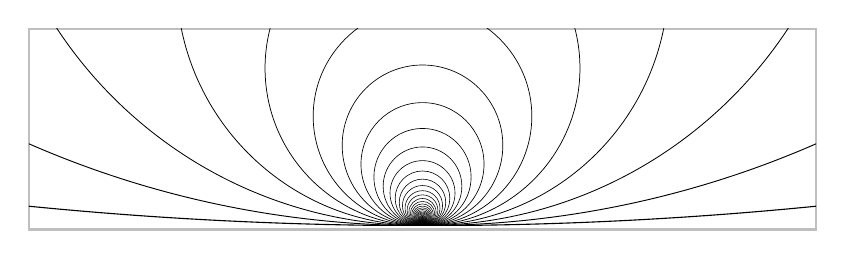
\begin{tikzpicture}[scale = 50]
			\draw[thick,lightgray] (-.1,-.001) rectangle (.1,.05);
			\clip (-.1,0) rectangle (.1,.05);
			\foreach \i in {1,...,100}{
				\draw[line width=0.4/\i^0.25 pt] (0, 1/\i^2) circle (1/\i^2);
			}
		\end{tikzpicture}
	\end{center}
	\smallskip
	\begin{equation*}
		\HE = \bigcup_{n \in \N} \left\{ (x_0, \dots, x_d) \in \R^{d+1} \ \middle | \ \left( x_0 - \frac{1}{n} \right)^2 \!\! + x_1^2 + \dots + x_d^2 = \left( \frac{1}{n} \right)^2 \right\}.
	\end{equation*}

	\medskip\pause

	\colorit{Example}.
	The function $f \colon \HE \to \R$ with
	\[
	f(\vec{x}) = \begin{cases}
		0, & \vec{x} = \vec{0}, \\
		1, & \vec{x} \neq \vec{0},
	\end{cases}
	\]
	is weakly $\HLC$ but $\rH(f_{\le})$ is not q-tame if $ \exists n$, $\dim \rH_{n}(\HE) = \infty$.
\end{frame}

\begin{frame}{Weak local connectivity and q-tameness}
	\pause
	\begin{minipage}{0.5\textwidth}
		\colorit{Definition.}
		$f \colon X \to \R$ is \colorit{locally homologically small} or $\HLC$ if for all $x \in X$, nbhd $V$ of $x$, and $f(x) < s < t$ there is a nbhd $U \subseteq V$ of $x$ s.t. $f_{\leq s} \cap U \to f_{\leq t} \cap V$ is $\HS$.
	\end{minipage}
	\begin{minipage}{0.4\textwidth}
		\hspace*{.5cm}\includegraphics[scale=.6]{aux/connectivity.pdf}
	\end{minipage}

	\bigskip\pause

	\begin{theorem}[BMS 2021]
		If $f$ is $\HLC$, then $\rH(f_{\le})$ is q-tame.
	\end{theorem}

	\smallskip\pause
	If so, it has a persistence diagram.
	This gives: \\
	a stable metric model of $X$ and generalized Morse inequalities.
\end{frame}

\begin{frame}{Morse--Tompkins proof}
	\colorit{Historical note}: To prove the Unstable Minimal Surface Theorem Morse and Tompkins needed the q-tameness of the sublevel set filtration of the space of surfaces.
	But their argument relied on a claim invalidated by our counterexample ($f \colon \HE \to \R$).

	\begin{displayquote}[Morse 1940]
		Let $a$ and $c$ be positive constants such that $a < c$.
		The $k^{\mathrm{th}}$ connectivity $R^k(a,c)$ of $F_a$ on $F_c$ is finite.
	\end{displayquote}

	Nonetheless, our second theorem ($\HLC \implies$ q-tame) applies to their situation so it can be used to ensures the assumed q-tameness.
\end{frame}

\begin{frame}{Conclusions}
	\pause
	Going from smooth compact Morse theory to functional topology:\\
	\medskip\pause
	\begin{enumerate}
		\item Work up to ephemeral information.\\
		\medskip\pause
		\item Barcodes replaced by persistent diagrams.\\
		\medskip\pause
		\item They exist for q-tame persistence modules.\\
		\medskip\pause
		\item They ensure stable metric model and generalized Morse inequalities.\\
		\medskip\pause
		\item $\rH(f_{\le})$ is q-tame if $f_{\le}$ is locally homologically connected.\\
		\medskip\pause
		\item Motivating example: the Douglas functional is $\HLC$.
	\end{enumerate}

\end{frame}
	%!TEX root = ../bgsu21.tex

{
	\usebackgroundtemplate{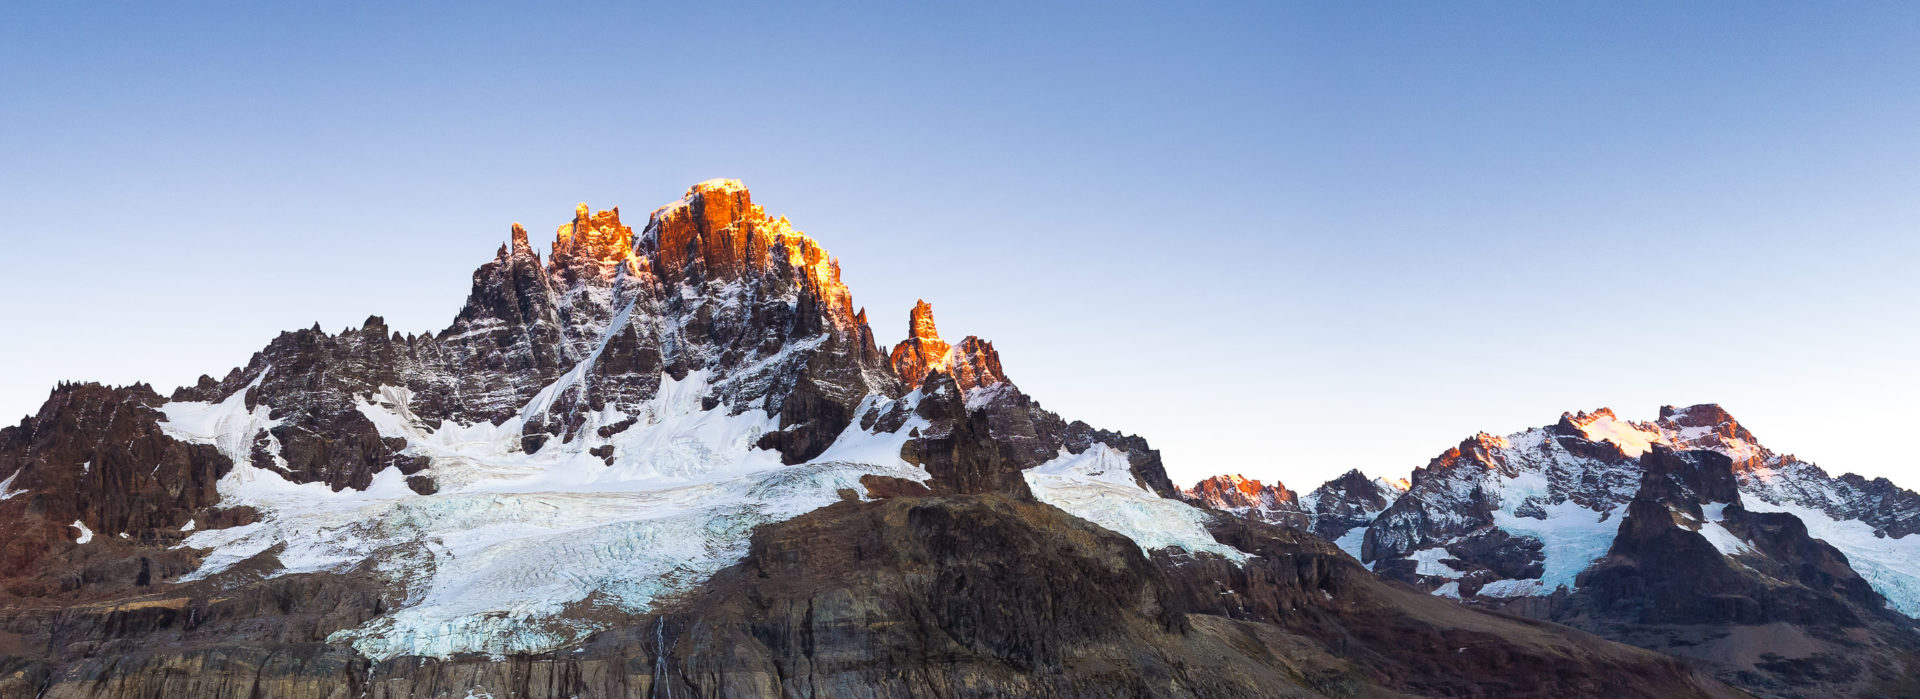
\includegraphics[width=\paperwidth]{aux/castillo.jpg}}%
	\begin{frame}
		\vskip 6cm
		\begin{center}
			\textcolor{pblue}{\Huge Thank you}
		\end{center}
	\end{frame}
}
\end{document}
